\documentclass{article} % For LaTeX2e
\usepackage{nips15submit_e,times}
\usepackage{hyperref}
\usepackage{url}
%\documentstyle[nips14submit_09,times,art10]{article} % For LaTeX 2.09
\usepackage[pdftex]{graphicx}  % omogoča vlaganje slik različnih 

\title{Neural network pruning with simultaneous matrix tri-factorization}
\author{Teja Roštan}
%\template is for anonymous submission

% The \author macro works with any number of authors. There are two commands
% used to separate the names and addresses of multiple authors: \And and \AND.
%
% Using \And between authors leaves it to \LaTeX{} to determine where to break
% the lines. Using \AND forces a linebreak at that point. So, if \LaTeX{}
% puts 3 of 4 authors names on the first line, and the last on the second
% line, try using \AND instead of \And before the third author name.

\newcommand{\fix}{\marginpar{FIX}}
\newcommand{\new}{\marginpar{NEW}}

%\nipsfinalcopy % Uncomment for camera-ready version

\begin{document}


\maketitle

\begin{abstract}
In this paper we present a novel approach for pruning neural network to reduce 
the model size and achieve better generalization performance. We apply a 
simultaneous matrix tri-factorization to map weight matrices to a 
low-dimensional space, therefore shrinking them and partially eliminating noise. 
Factorized models are thus more robust and have a better generalization 
ability...
\end{abstract}

\section{Introduction}
Deep neural networks are a popular tool used to solve a certain problem. The 
advantages of neural networks are that they are relatively easy to use and can 
approximate any function, regardless of its linearity. They are widely used for 
complex or abstract problems such as image, sound and text recognition. However, 
they are computationally intensive to train and are known for black box problem 
as they will not tell you why they reached a certain conclusion. Success of 
neural networks largely depends on their architecture. While the size of the 
input layer and the output layer is known, the number of hidden layers and the 
number of nodes in each hidden layer depends on the complexity of the 
problem~\cite{augasta2013pruning}. Generally, a network with large number of 
hidden nodes is able to learn fast and avoids local minima, but when a network 
is oversized, the network may overfit the training data and lose its 
generalization ability while still having unnecessary calculations as they are 
using more nodes than necessary.  Better generalization performance can be 
achieved only by small networks. They are easier to interpret but their training 
may require a lot of effort. Also too small networks are very sensitive to 
initial conditions and learning parameters and are prone to not learn the given 
problem. The most popular approach to obtain the most optimal architecture of 
neural network is pruning. Pruning is defined as a network trimming within the 
assumed initial architecture, which is larger than necessary. Pruning algorithms 
are used to remove the redundant connections while maintaining the networks 
performance. So one can use the larger networks for training and its 
generalization can be improved by the process of 
pruning~\cite{augasta2013pruning}.

More recent researches have tackled upon an issue of deep neural network and 
deep convolutional neural networks which is that they involve many layers with 
millions of parameters, making the size of the network model to be extremely 
large to store. This prohibits the usage on resource limited hardware especially 
mobile devices or other embedded devices even though deep neural networks are 
increasingly used in applications suited for mobile 
devices~\cite{DBLP:journals/corr/GongLYB14}.

In this work we present a novel approach using low-dimensional matrix 
factorization. Because we have more than one weight matrix and because the 
weight matrices between the layers in a neural network are dependent with their 
neighbor matrices, we used an upgraded approach of matrix factorization, named 
simultaneous matrix tri-factorization, or in other words, data fusion. Pruning 
neural network with simultaneous matrix tri-factorization was names as matrix 
factorization-based brain pruning (MFBP).

\section{Related work}
In article~\cite{denil2013predicting} they said that giving only a few weight 
values for each feature it is possible to accurately predict the remaining 
values while many of them do not need to be learned at all. They exploited the 
fact that the weights in learned networks tend to be sparse and structured.
Another article~\cite{augasta2013pruning} have shown that, in any case the 
overall time required for training a large network and then pruning it to a 
small size compares very favorably with that of simply training a small network. 
 
Because there 
is significant redundancy in the parametrization of networks, many researchers 
found solutions to prune neural networks with possible accuracy loss in order to 
reduce the model size extensively. But were able to fine-tune the compressed 
layers with added learning iterations to recover the performance and improve the 
accuracy back. 

Compressing the most storage 
demanding dense connected layers is possible by neural network pruning with 
low-rank matrix factorization methods~\cite{bondarenko2014artificial, 
schmidhuber2015deep, sainath2013low}, where network pruning has been used both 
to reduce model size and to reduce over-fitting~\cite{han2015learning}. 
State-of-the-art approaches are Optimal Brain Damage~\cite{lecun1989optimal} and 
Optimal Brain Surgeon~\cite{hassibi1993optimal} which open the rich field of 
studies using matrix factorization to prune the networks. 

Besides neural network pruning with matrix factorization many alternatives have 
been used in numerous ways to optimize neural network architecture. One of the 
latest study~\cite{DBLP:journals/corr/GongLYB14}used vector quantization methods 
for which they said have a clear gain over existing matrix factorization 
methods. Alternative approach~\cite{xue2013restructuring}is application of 
singular value decomposition (SVD) on the weight matrices to decompose them and 
reconstruct the model based on the sparseness of the original matrices. There 
were also studies which used evolutionary pruning, more precisely, Genetic 
Algorithms~\cite{li2012tuning} to examine potential redundancy in data and 
therefore prune the neural network. A simple solution to reduce the model size 
and preserve the generalization ability is to train models that have a constant 
number of simpler neurons which was presented in 
article~\cite{collins2014memory}.

Another examined strong method uses the significance of neurons by evaluating 
the information on weight variation and consequently prune the insignificant 
nodes. 
Removing all connections whose weight is lower than a threshold is introduced 
in~\cite{han2015learning}. There the first phase learns which connections are 
important and removes the unimportant ones using multiple iterations. Hashing is 
also an effective strategy for dimensionality reduction while preserving 
generalization performance~\cite{weinberger2009feature, shi2009hash}. The 
strategy used on neural networks named HashedNets~\cite{chen2015compressing} 
uses a low-cost hash function to randomly group connection weights into hash 
buckets where all connection inside share a single and tuned parameter value. 

Compressing the parameters to reduce model size brings the focus upon how to 
prune the dense connected layers since the vast majority of weights reside in 
these layers which results in significant savings and by replacing the fully 
connected layers of the network with an Adaptive Fastfood transform, introduced 
in article~\cite{yang2014deep}, and results 
in a deep fried convnet. The Fastfood transform allows for a theoretical 
reduction in computation also. However, the computation in convolutional neural 
networks is dominated by the convolutions, and hence the deep fried convnets are 
not necessarily faster in practice. 
%In convolutional neural network, about 90\% 
%of the model size is taken up by the dense connected layers and more than 90\% 
%of the running time is taken by the convolutional 
%layers~\cite{zeiler2014visualizing}. 

%Running time complexity is depended from the computation which is dominated by 
%convolution operations in the lower layers of the model. In contrast to model 
%size compression, fewer approaches focused on reducing the time complexity. One 
%of the earlier approaches of reducing the 
%time complexity is FFT algorithm~\cite{mathieu2013fast} which by computing the 
%Fourier transforms of the matrices in each set efficiently performs convolutions 
%as pairwise products. Main disadvantage of this approach is that in current 
%implementation of the FFT algorithm, input images which
%are not a power of 2 must be padded to the next highest power. In newer 
%researches they exploit the redundancy 
%that exists between different feature channels and filters. In 
%articles~\cite{jaderberg2014speeding, rigamonti2013learning} they use an
%intuition that CNN filter banks can be approximated using a low rank basis of
%filters that are separable in the spatial domain where 
%in~\cite{jaderberg2014speeding}
%substantial speedups can be achieved by also exploiting the cross-channel 
%redundancy to perform low-rank decomposition in the
%channel dimension as well. Alternatively in article~\cite{denton2014exploiting} 
%they compressed each 
%convolutional layer by finding an appropriate low-rank approximation with 
%considering several elementary tensor decompositions based on singular value 
%decompositions, as well as filter clustering methods to take advantage of 
%similarities between learned features.

\section{Method description}
\begin{figure}[!ht]
\centering
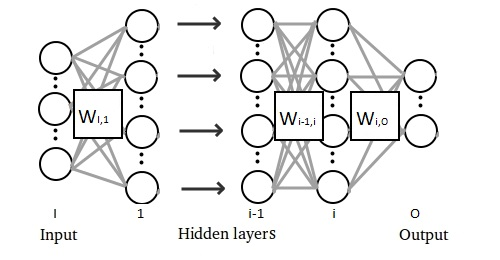
\includegraphics[width=.75\textwidth]{globokamreza2.jpg}
\caption{Deep neural network with densed connected layers.}
\label{f:globokamreza}
\end{figure}
Deep neural network is a feed-forward, artificial neural network with more than 
one or two hidden layers between the input and output layer. 
Figure~\ref{f:globokamreza} shows the structure of a deep neural network. The 
number of nodes on the left layer, known as the input layer, is the same as the 
number of attributes in a dataset while the number of nodes in the most right 
layer, named as output layer is the same as the number of classes. Between them 
are the hidden layers as mentioned above. The number of nodes in every hidden 
layer is depended of the dataset we used. Our main goal was to use more nodes 
than necessary to prune the unnecessary ones later.

\subsection{Approximation of matrix with matrix factorization}
Matrix factorization is a technique to search linear representation with 
factorizing. Approximation of matrix with matrix factorization is used to 
approximate the data in low-dimensional space in order to find latent features. 
The theorem of the method matrix factorization follows:

Izrek: Given is a matrix $A \in \Re^{m \times n}$ and a positive integer $k \ll 
min\{m,n\}$. Find matrices $W \in \Re^{m \times k}$ and $H \in \Re^{k \times 
n}$, such that $WH \approx A$. the product $WH$ is named as a matrix 
factorization (MF) of a matrix $A$. $WH$ is an approximated factorization if 
rang $r = k$.

We assume that factorized matrix $W$ has less columns than the original matrix $A$ 
has rows. Approximation is successful only when the latent structure is found 
and the dimensionality of data gets lower. Applications, such as text 
processing, image processing and data mining store valuable information in very 
big matrices. Not only that low rank matrix factorization reduces the 
consumption of memory but also offers more clear and more efficient 
representation of connections between data~\cite{neyshabur2013sparse}. A low 
rank approximation finds the key components of data and discards the data that 
attribute to noise, error or inconsistency~\cite{langville2014algorithms}. 
Because of the potential of matrix factorization, a lot of upgraded versions 
were created. One of them is a simultaneous matrix 
factorization~\cite{zitnik2015data}.

\subsection{Simultaneous matrix tri-factorization}
Izrek: Simultaneous tri-factorization of multiple matrices simultaneously 
factorize all available relation matrices $R_{ij}$ v $G_i € \Re^{n_i \times 
k_i}$, $G_j E \Re^{n_j \times k_j}$ in $S € \Re^{k_i \times k_j}$ and regulize 
their approximations through constrained matrices $\theta_i$ and $\theta_j$, 
such that $R_{ij} \approx G_iS_{ij}G_j^T$~\cite{zitnik2015data}. 

Simultaneous matrix tri-factorization focuses on a specific target relation and 
exploits directly connected data. It contains a set of restrictions of the 
connections that should connect and of those which should not. In that way it 
contains the relations between the objects of the same 
type~\cite{zitnik2015data}. It finds latent associations between matrices with 
simultaneous factorization of matrices, therefore directly considers every 
dataset that can be represented as a matrix~\cite{zitnik2015data}.

\begin{figure}[!ht]
\centering 
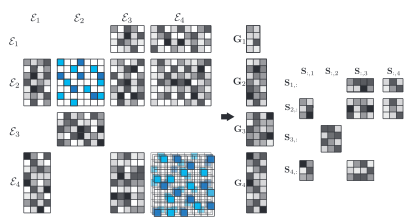
\includegraphics[width=.8\textwidth]{Izbor_037.png}
\caption{An example of simultaneous matrix tri-factorization. 
On the left side are all available relation matrices $R$. 
They are factorized to matrices $G$ and $S$ (on the right). 
Source~\cite{zitnik2015data}.}
\label{f:zlitje_matricne_tri-faktorizacije}
\end{figure}

The data fusion algorithm considers $r$ object types $\xi_1,…,\xi_r$ and a 
collection of data sources, each relating a pair of object types 
$(\xi_i,\xi_j)$. If there are $n_i$ objects of type $\xi_i$ and $n_j$ objects of 
type $\xi_j$, it represents the observations from the data source that relates 
$(\xi_i,\xi_j)$ or $i \neq j$ in a sparse matrix $R_{ij} € \Re^{n_i \times 
n_j}$. In general matrices $R_{ij}$ and $R_{ji}$ need not be symmetric. A data 
source that provides relations between objects of the same type $\xi_i$ is 
represented by a constrant matrix $\theta_i \in \Re^{n_i \times 
n_i}$~\cite{zitnik2015data}.  
Even if we are missing relations between some pairs, the algorithm still 
integrates all available data if an underlying graph of relations between object 
types is connected. Figure~\ref{f:zlitje_matricne_tri-faktorizacije} shows an 
example of a block configuration of the fusion system with four object 
types~\cite{zitnik2015data}.

To retain the block structure of a system, it is proposed the simultaneous 
matrix tri-factorization of all relation matrices $R_{ij}$ constrained by 
$\theta_i$. The resulting system contains factors that are specific to each data 
source and factors that are specific to each object type. Through factor sharing 
it fuses the data but also identifies source-specific 
patterns~\cite{zitnik2015data}.
\subsection{Matrix factorization-based brain pruning}
With ordinary artificial neural network, we have only one hidden layer and 
therefore two weight matrices with the same object type (sharing dimension). 
Because of this property, we are able to concatenate the matrices through 
sharing dimension and apply a matrix factorization. With deep neural networks we 
have a multi-layer architecture where neighbor weight matrices share the same 
object type (same dimension).  We can apply co-dependency between neighbor 
weight matrices but we can apply dependency between, for example, first and 
third weight matrix. With simultaneous matrix tri-factorization we can solve the 
mentioned problem and pruning neural networks with simultaneous matrix 
tri-factorization named matrix factorization-based brain pruning (MFBP).

\begin{figure}[!ht]
\centering
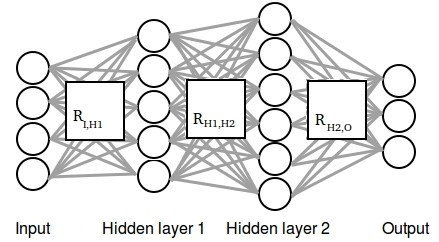
\includegraphics[width=10cm]{mrezafusion.jpg}
\caption{Artificial two-layered neural network with weight matrices (relation 
matrices $R$).
The size od each matrix is dependent by number of neurons on surrounding layers. 
For example $R_{I,H1}$ has four ($I$) rows and five ($H1$) columns.}
\label{f:mrezafusion}
\end{figure}

\begin{figure}[!ht]
\centering 
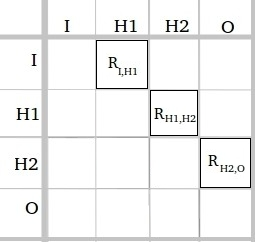
\includegraphics[width=2.2in]{tabelafusion.jpg}
\caption{Configuration of relation matrices $R$ from figure~\ref{f:mrezafusion} 
for simultaneous matrix tri-factorization. In our case, 
the relation matrices $R$ present weight matrices of neural network.
Configuration is set on diagonal because the neighbour weight matrices share the 
dimension
from shared hidden layer}
\label{f:tabelafusion}
\end{figure}  
In a figure~\ref{f:mrezafusion} is shown a neural network with two hidden layers 
and relation weight matrices $R$ between them. The weight matrices are collected 
from neural network and configured in a graph of relations as shown in 
figure~\ref{f:tabelafusion}. The graph of relations is then used in data fusion. 
The result are approximations of the weight matrices. With approximations we 
determined which weights are better to prune. In theory it is said that a weight 
is pruned, when its value equals zero. But because in practice the weights are 
almost always non-zero, we have to estimate which weights to prune.

\begin{figure}[!ht]
\centering 
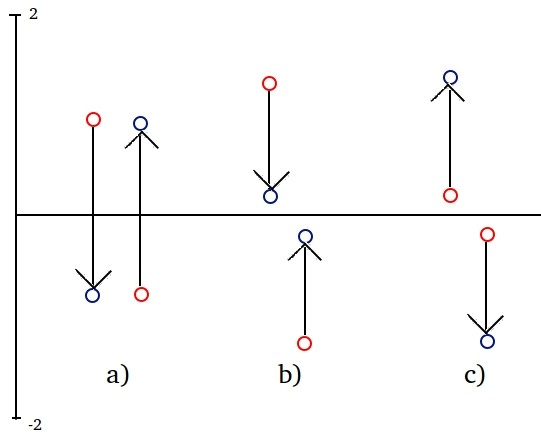
\includegraphics[height=4.5cm]{kriterijrezanja.jpg}
\caption{Possible changes of values of weights. Values before pruning (red 
circle) and after pruning (blue circle). In a) case, the weight value changes 
sign, b) moves closer to zero and c) moves away from zero.}
\label{f:spremembeutezi}
\end{figure}
In figure~\ref{f:spremembeutezi} are shown possible changes that can happen 
after data fusion. A weight can change its sign, can move closer to zero or move 
away from it. We chose the weights where absolute value move closer to zero for 
enough amount (for 0.2 in our case) for pruning. We set the chosen weights to 
zero and keep them at that value. Below is shown a pseudocode of our algorithm.

… Pseudocode …

\section{Experimental setup}
We evaluated matrix factorization-based brain pruning on MNIST (Mixed National 
Institute of Standards and Technology dataset) dataset. The MNIST database of 
handwritten digits 0-9, available in~\cite{lecun-mnisthandwrittendigit-2010}, 
has a training set of 60,000 instances and a test set of 10,000 instances. The 
digits have been size-normalized and centered in a fixed-size 28x28 images. 

We used a “modern” neural network, presented in~\cite{github}. There are two 
main contributions to a modern neural network. One is changing of activation 
function. Instead of sigmoid function it uses a rectifier (Rectified linear unit 
(ReLU) $f(x) = max(0, x)$, where $x$ is the input to a neuron. What the 
rectifier does is that if the input to a neuron is below zero the activation 
function does nothing. If the input is above zero it does activate. This 
activation function has been argued to be more biologically 
plausible~\cite{AISTATS2011_GlorotBB11}. It induces the sparsity in the hidden 
neurons. Another advantage of rectifier is that it does not face gradient 
vanishing problem as with sigmoid or tanh function. It has ben also shown that 
can be deep neural networks trained efficiently using rectifier even without 
pre-training. The other contribution is regularizing the model with 
dropout~\cite{srivastava2014dropout}. Dropout is one of the biggest improvements 
in the field of neural networks in recent years as it addresses the main problem 
in deep learning that is overfitting. The purpose of dropout is to add some 
noise by “dropping out” a random number of some neuron activations in a given 
layer. By dropping them is meant to set them to zero or as in our case to prune 
them. With every iteration a different random set of neurons are chosen to drop, 
therefore it prevents co-adaptation of neurons. 
There was also a change at update rule. Instead of a standard stochastic 
gradient descent (SGD) backpropagation method we used RMSprop (A mini-batch 
version of rpop). The idea behind SGD is to approximate the real update step by 
taking the average of the all given instances or as in our case mini batches. 
The problem of SGD is that it is sensitive to outliers which can destroy all the 
gradient information collected before~\cite{erogol}. On the other hand, the 
RMSprop keeps a running average of its recent gradient magnitudes and divides 
the next gradient by this average so that loosely gradient values are 
normalized~\cite{lecture}. RMSprop follows: 
$MeanSquare(w, t) = 0.9 MeanSquare(w, t-1) + 0.1 {({\delta E}/{\delta 
w^{(t)}}}^2$~\cite{lecture}.


To evaluate our experiments, we implemented algorithm on Python with the help of 
Theano~\cite{Bastien-Theano-2012, bergstra+al:2010-scipy}. Theano is a Python 
library that is suitable for building an optimized neural network. We chose it 
as it gives a comprehensive control over neural network formation which is 
suitable for our problem. Another reason we used Theano is because the 
implementation of “modern neural net” described above is available online as 
open source. Data fusion algorithm which performs simultaneous matrix 
tri-factorization is available in a python library 
Scikit-fusion~\cite{zitnik2015data}. To measure our results, we used a machine 
learning library Scikit-learn~\cite{scikit-learn}. 

To estimate and analyze our results, we trained and tested four neural networks: 
ordinary neural network with two hidden layers without pruning, ordinary neural 
network with two hidden layers with pruning, deep neural network with five 
hidden layers without pruning and another deep neural network with five hidden 
layers with pruning. Every neural network had 60 iterations available to learn. 
The non-pruned networks learned on 60 iterations where every iteration had 
50,000 train instances packed in mini-batches of 128. The pruned network had 40 
iterations to learn without pruning. The other 20 iterations consisted of every 
second iteration of pruning (overall 10 iterations of pruning) and another half 
of iterations for fine-tuning. Fine-tuning was used to adapt the non-pruned 
weights which have been affected with pruning, in other words, to recover the 
non-pruned weight values which have been biased by the pruned weights before 
pruning. In this case there were also all 50,000 train instances available at 
every iteration in mini-batches.

\section{Results}
The reported results are measured with area under ROC curve (AC) on test set 
and shown in figure~\ref{f:results}. The model size compression rate in \% 
results are coming...
\begin{figure}[!ht]
\centering
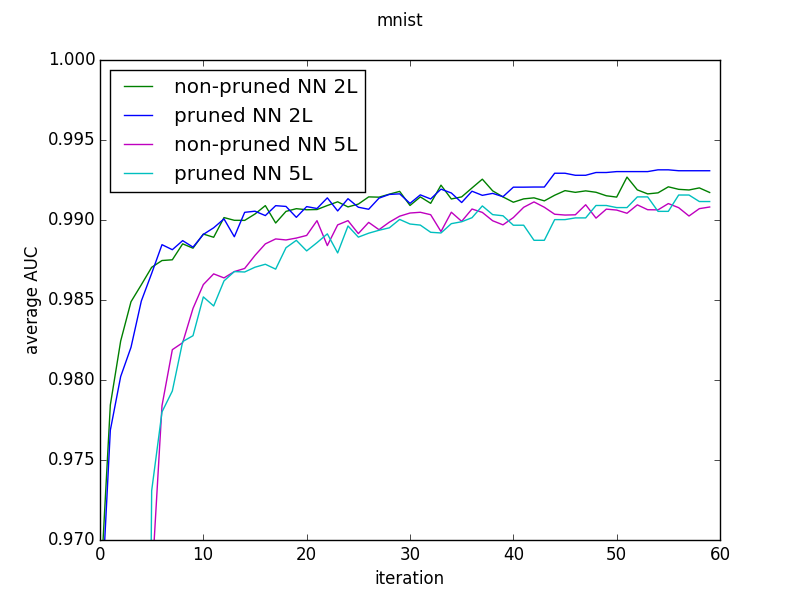
\includegraphics[width=10cm]{mnist2.png}
\caption{AUC results of neural networks. With pruned neural networks, the 
pruning starts at 40th iteration.}
\label{f:results}
\end{figure}



\section{Discussion and conclusion}
To be written...


\subsubsection*{Acknowledgments}



\subsubsection*{References}
\bibliography{literature}
\bibliographystyle{plain}
%\small{
%[1] Alexander, J.A. \& Mozer, M.C. (1995) Template-basedalgorithms
%for connectionist rule extraction. In G. Tesauro, D. S. Touretzky
%and T.K. Leen (eds.), {\it Advances in Neural Information Processing
%Systems 7}, pp. 609-616. Cambridge, MA: MIT Press.

%[2] Bower, J.M. \& Beeman, D. (1995) {\it The Book of GENESIS: Exploring
%Realistic Neural Models with the GEneral NEural SImulation System.}
%New York: TELOS/Springer-Verlag.

%[3] Hasselmo, M.E., Schnell, E. \& Barkai, E. (1995) Dynamics of learning
%and recall at excitatory recurrent synapses and cholinergic modulation
%in rat hippocampal region CA3. {\it Journal of Neuroscience}
%{\bf 15}(7):5249-5262.
%}

\end{document}
